\documentclass[conference]{IEEEtran}
\IEEEoverridecommandlockouts
% The preceding line is only needed to identify funding in the first footnote. If that is unneeded, please comment it out.
%\usepackage{cite}
\usepackage{amsmath,amssymb,amsfonts}
\usepackage{algorithmic}
\usepackage{graphicx}
%\usepackage{textcomp}
\usepackage{xcolor}
\usepackage{subfig}
\usepackage{multirow}
\usepackage{booktabs}
\usepackage{tabularx}

\usepackage[nomain, toc, acronym]{glossaries}
%\glsdisablehyper

\newcommand\note[2]{{\color{#1}#2}}
\newcommand\todo[1]{{\note{red}{TODO: #1}}}

%\newcommand{\unsw}{UNSW-NB15}
%\newcommand{\cic}{CIC-IDS-2017}

\newacronym{dl}{DL}{Deep Learning}
\newacronym{ad}{AD}{Anomaly Detection}
\newacronym{ml}{ML}{Machine Learning}
\newacronym{ttl}{TTL}{Time-to-Live}
\newacronym{ids}{IDS}{Intrusion Detection System}
\newacronym{mlp}{MLP}{Multilayer Perceptron}
\newacronym{relu}{ReLU}{Rectified Linear Unit}
\newacronym{ip}{IP}{Internet Protocol}
\newacronym{ffnn}{FNN}{Feedforward Neural Network}

\begin{document}

%\title{EagerNet: Early Intrusion Prediction\\in Feed Forward Neural Networks}
%\title{EagerNet: Early Predictions in Feedforward Neural Networks for Fast Network Intrusion Detection}
% Max Proposal
\title{EagerNet: Early Predictions of Neural Networks for Computationally Efficient Intrusion Detection}

\author{\IEEEauthorblockN{Fares Meghdouri, Maximilian Bachl and Tanja Zseby}
\IEEEauthorblockA{Technische Universität Wien\\
Vienna, Austria\\
firstname.lastname@tuwien.ac.at}}



\maketitle

\begin{abstract}

\glspl{ffnn} have been the basis of most state-of-the-art \gls{ml} applications in recent years. Experiments show that the deeper the network is, the more desirable it is to acquire more knowledge. Nonetheless, with the growing number of layers, obtaining fast predictions has become a difficult task despite the use of special hardware such as GPUs. We propose a new architecture to obtain predictions without conducting a forward-pass until the last layer. The architecture is able to deal with either binary or multiclass classification problems and trades prediction speed for the confidence of the network. We evaluate our proposal with two different network intrusion detection datasets. Results suggest that it is possible to obtain comparable accuracies to simple \glspl{ffnn} without evaluating all layers, thus obtaining early predictions and saving energy and computational efforts.

\end{abstract}

\begin{IEEEkeywords}

\end{IEEEkeywords}

\section{Introduction}
% what are ffnn
\glspl{ffnn} have gained remarkable attention in recent years due to the availability of data and computational resources for research. Many of the state-of-the-art architectures currently used in different applications are effectively based on simple \glspl{ffnn} architectures. Experiments show that the more layers (and neurons) the network includes, the more desirable it is for better learning \cite{eldan_power_2016} .

% forward-backward
Traditional \gls{ffnn} are based on simple logistic regression units that combine multiple inputs multiplied by a set of weights and passed through an activation function (e.g. sigmoid) to obtain a scalar. The weights are adjusted to give the closest possible output to a ground-truth. As far as neural networks are concerned, logistic regression units are stacked together to create layers and then layers are stacked together again to create the network itself. Figure \ref{fig:ffnn} demonstrates a basic \gls{ffnn} that utilizes the input vector $\lbrace x_{1}, x_{2} ... x_{m} \rbrace$ and makes a prediction. Adjusting weights in such situations is a non-trivial problem since the weights of each layer may have an impact on the previous layers. Fortunately, several algorithms have been proposed to reduce the complexity of the task (e.g. gradient descent learning) while achieving the same goal: reduce the "gap" (loss) between predictions and actual desired output. Larger networks consist of more neurons and thus more weights, allowing more data patterns to be learned.

% problem with large networks
In terms of efficiency, two problems arise when using an extremely deep neural networks: (1) The loss during training needs more time to converge and (2) prediction time is proportional to the number of layers. Even though most modern hardware is able to cope with offline single predictions without significant delay, online massive neural network implementations may suffer from the latter issue if non-specialized hardware is used to produce predictions.
%EagerNet
To solve this, we propose a new architecture that, on the one hand, uses the entire network capacity for learning and, on the other hand, stops the forward-pass and makes predictions as soon as confidence reaches a certain threshold. In other words, it makes it possible to avoid evaluating the entire network and to receive predictions from intermediate layers with the same performance of a simple \gls{ffnn}. The proposed approach therefore allows, where possible, the reduction of computing resources and energy usage preserving comparable performance of a full forward-pass.

% talk about network traffic

% conclusion
The rest of the paper is organized as follows: In Section ...

\section{Related Work}



 \begin{figure}
  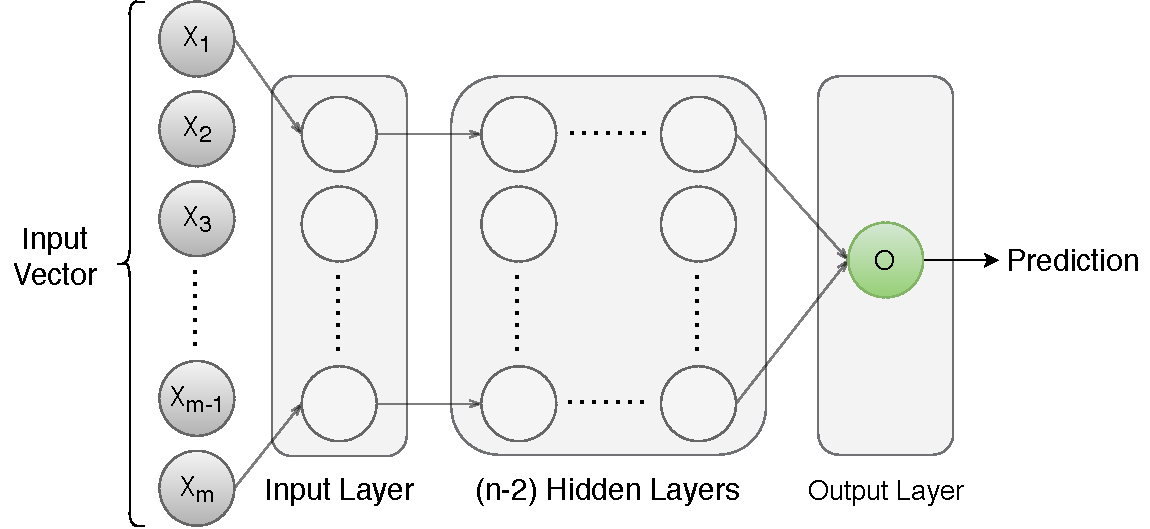
\includegraphics[width=\linewidth]{figures/ffnn_new.pdf}
  \caption{Conventional \gls{ffnn} architecture.}
  \label{fig:ffnn}
\end{figure}

\section{Supervised Learning for Network Intrusion Detection}

\gls{ml} has been widely used in the last decade for network traffic analysis and specifically anomaly detection systems. Many of the works proposed \gls{ids} architectures based on well-known supervised techniques \cite{survey}. The idea of training a classifier on pre-stored attack patterns and using the same classifier to recognize similar patterns is commonly used and remarkable success has so far been achieved \cite{survey}. In particular, \glspl{ffnn} is commonly used whenever large amounts of data are available. In order to present network data to such architectures, a number of traffic representation families have been proposed depending on the application. However, the statistical representation of flow characteristics is still the most appropriate. In this work, we define the network flow to be the exchange of packets between two end-hosts. Packets can be identified and aggregated using the five-tuple key: \emph{sourceIP}, \emph{destinationIP}, \emph{sourceTransportPort}, \emph{destinationTransportPort} and \emph{protocolIdentifier}. Thereafter, packet features are extracted and the statistical combinations are computed. Table \ref{tab:features} shows CAIA \cite{williams_preliminary_2006} network traffic representation. It consists of 12 features 7 of which are measured in both directions and 2 of which are expanded using four statistical combinations (i.e. \emph{A} becomes \emph{mean(A)}, \emph{min(A)}, \emph{max(A)} and \emph{stdev(A)}). In addition, we set an observation timeout of 1,800 seconds, after which we terminate flows. Each flow is considered to be a data sample and has two sets of labels: binary (attack/benign) label and attack family. After a training process, the trained \gls{ids} must be able to correctly classify new flows.

\begin{table}[ht!]

	\centering
	\caption{CAIA flow representation.}
	\label{tab:features}

	\footnotesize
	\begin{tabular}{|c|c|c|}
		\hline
		\textbf{Direction}                    & \textbf{Features}        & \textbf{Statistical Operations}        \\
		\hline

		                                      & flowDurationMilliseconds &                                        \\
		                                      & sourceTransportPort      &                                        \\
		                                      & destinationTransportPort &                                        \\
		                                      & protocolIdentifier       &                                        \\
		                                      & octetTotalCount          &                                        \\
		\hline
		\multirow{7}{*}{\shortstack{Forward and\\ Backward}} & ipTotalLength            & \multirow{2}{*}{Mean, Min, Max, Stdev} \\
		                                      & interPacketTimeSeconds   &                                        \\
		\cline{2-3}
		                                      & packetTotalCount         &                                        \\
		                                      & tcpSynTotalCount         &                                        \\
		                                      & tcpAckTotalCount         &                                        \\
		                                      & tcpFinTotalCount         &                                        \\
		                                      & tcpCwrTotalCount         &                                        \\

		\hline


	\end{tabular}

\end{table}

\section{EagerNet}

Because several network attack families are simple to detect on the basis of linear input combinations, the standard \gls{ffnn} is slightly modified to cope with the difficulty of detection. Our novel architecture is based on the assumption that deep neural networks can learn complex functions with simpler mappings learned in the first few layers. As a result, we build a network such that an additional set of neurons is connected to each layer (a copy of the output layer), allowing for predictions at each layer. The EagerNet architecture is shown in Figure \ref{fig:eagerNet_forward}. Initial neurons are shown in gray and output neurons (per layer) are shown in green. Once a flow is observed and features are extracted, a sample $\textbf{X}$ is fed to the network via the input layer. The network proceeds evaluating the output of each layer and yields a prediction confidence value. We define the confidence as the value that represents how sure the network is about a certain decision or sample belonging to a certain class. Based on a predefined threshold, the network measures confidence and determines whether to avoid testing additional layers or proceed to do so in order to gain more confidence. This methodology ensures that simpler samples are classified early in the forward-pass and that more complicated, noisy samples are passed into deeper layers. In the \ref{confidence-speed-tradeoff} Section, we show that EagerNet reduces resource consumption on average keeping comparable performance to normal \gls{ffnn}.


\begin{figure*}[htp]
\center

\subfloat[EagerNet: Forward-pass.]{%
  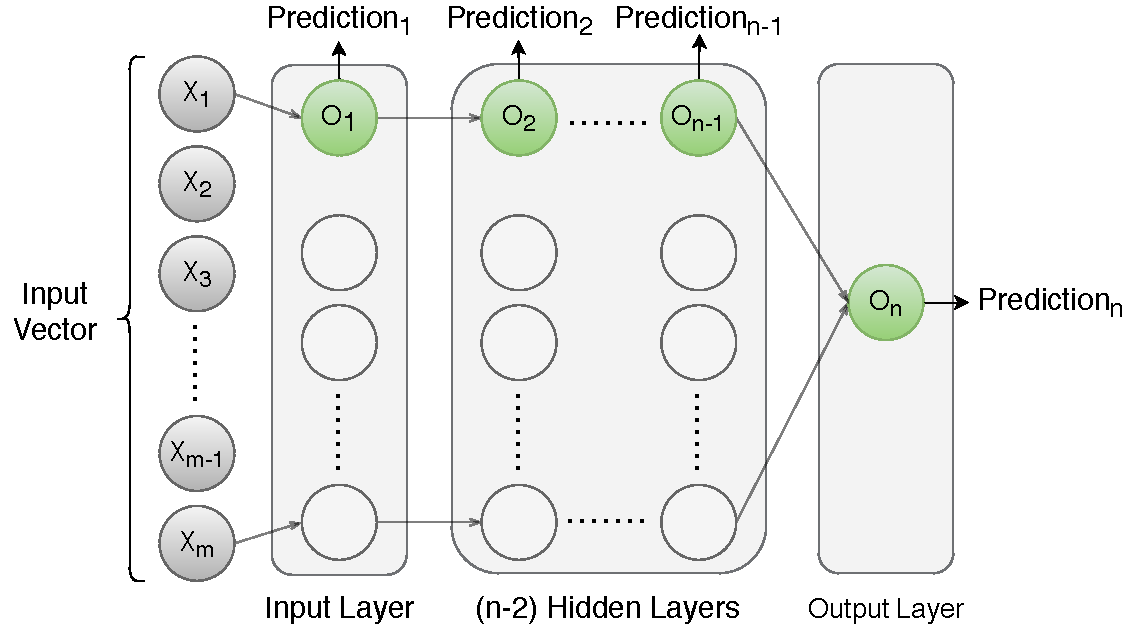
\includegraphics[clip,width=0.5\textwidth]{figures/eagernet_new.pdf}%
  \label{fig:eagerNet_forward}
}
\quad
\subfloat[EagerNet: Back-propagation of gradients.]{%
  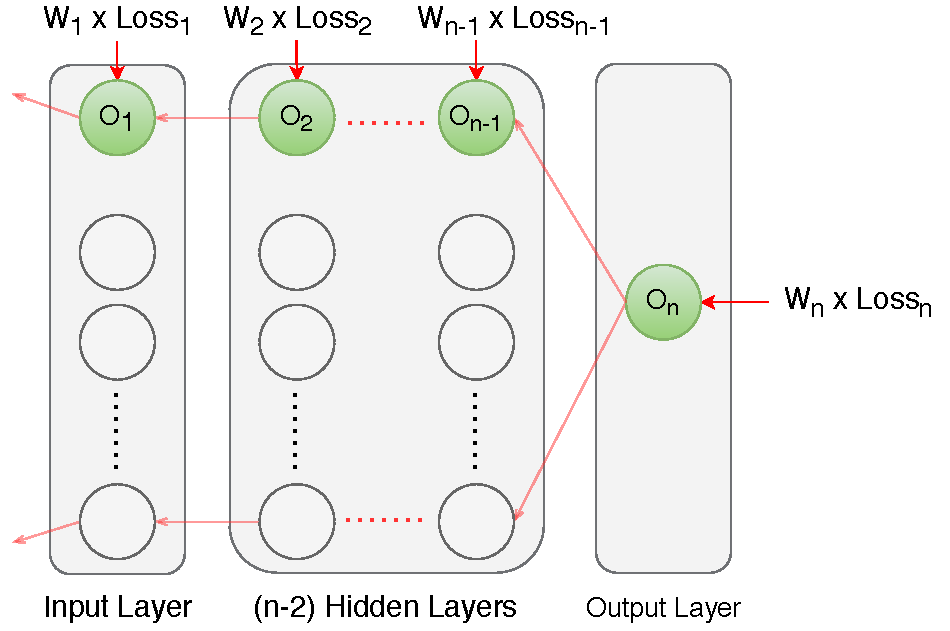
\includegraphics[clip,width=0.42\textwidth]{figures/eagernet_backprop_new.pdf}%
  \label{fig:eagerNet_backward}
}

\caption{The difference between conventional neural networks and our proposed architecture.}

\end{figure*}

\subsubsection{Binary Vs. Multiclass Classification}
We adjust the output layer to build two separate sub-architectures. The first architecture, consisting of a binary attack detection, i.e. a 1 is an attack flow and a 0 is a benign flow. The predictions in this case are given by a single output neuron followed by a sigmoid activation function to force values between 0 and 1. During back-propagation, we use a binary cross-entropy loss including the activation function and average the loss over the batch. Equation \ref{eq:bceloss} shows how the loss is determined for a batch of size $N$, with the $n^{th}$ input $x_{n}$ and the sigmoid activation function  $\sigma(.)$.

\begin{equation}
\label{eq:bceloss}
l = - \frac{1}{N} \sum_{n}^{N} [y_n \cdot \log \sigma (x_{n}) + (1 - y_n) \cdot \log (1 - \sigma (x_{n}))]
\end{equation}

In the case of a multiclass problem, the output layers consist of as many neurons as attack families followed by a softmax activation functions that allow at most only one neuron to be 1. During back-propagation, we use the categorical cross-entropy loss to penalize all outputs together, so there is no overlap between classes. Equation \ref{eq:cceloss} shows how the loss is determined for a batch of size $N$, with the $n^{th}$ input $x_{n}$ and the softmax activation function  $\phi(.)$, $C$ being the number of classes or output neurons and $i$ is the current class/output.

\begin{equation}
\label{eq:cceloss}
l = - \frac{1}{N} \sum_{n}^{N} \sum_{i}^{C} y_{n,i} \cdot \log (\phi(x_{n})_{i})
\end{equation}

After computing the losses, we use $Adam$ optimizer \cite{kingma_adam_2017} for computing gradients with a learning rate of 0.001.


\subsubsection{Combined Back-propagation Loss}
Conventional \gls{ffnn} uses the loss of the last layer to adjust the gradients. In this research, and since we have multiple outputs; one at each layer, we aggregate the losses and back propagate them. Fig \ref{fig:eagerNet_backward} demonstrates how losses propagate back from the respective layer only. As a consequence, the weights of the last layer are affected only by the loss of the last output. Similarly, the weights of the first layer are affected by the losses of the entire network. In addition, we introduce a weighting policy for losses. We allocate a weight to each loss that is predefined prior to training. The aim is to help the network determine on which layer to optimize more. Three types of weight sets are defined:
\begin{itemize}
\item Uniform weights. all losses have the same weight:
\begin{equation}
\mathcal{W_U} = \lbrace W_{0}, ..., W_{n} \rbrace = \lbrace \frac{1}{\sum_{i=0}^{n} 1}, ..., \frac{1}{\sum_{i=0}^{n} 1} \rbrace
\end{equation}

\item Increasing weights. losses are increasingly important from first to last layer.
\begin{equation}
\mathcal{W_I} = \lbrace W_{0}, ..., W_{n} \rbrace = \lbrace \frac{1}{\sum_{i=0}^{n} i+1}, ..., \frac{n+1}{\sum_{i=0}^{n} i+1} \rbrace
\end{equation}

\item Decreasing weights. losses are decreasingly important from first to last layer.
\begin{equation}
\mathcal{W_D} = \lbrace W_{0}, ..., W_{n} \rbrace = \lbrace \frac{n+1}{\sum_{i=0}^{n} i+1}, ..., \frac{1}{\sum_{i=0}^{n} i+1} \rbrace
\end{equation}

\end{itemize}

We show the effect of the weight distributions in Table \ref{tab:weights} and discuss results in Section \ref{evaluation_and_discussion}.

%\begin{equation}
%\nabla l = {\underbrace{W_{current} \times \nabla l_{current}}_{\text{Current gradient}}} + {\underbrace{\sum_{i}^{} \nabla l_{i}}_{\text{Next layer gradients}}}
%\end{equation}

%\subsubsection{Enhanced Training}
%Back-propagating all losses together even when using weighted-loss summation causes the network to minimize the loss on each layer hence learning all classes at each layer simultaneously if the training procedure is long enough thus causing (1) the first few layers to over-fit and (2) the network's loss to converge slowly if there are many classes to learn. To solve this issue, we propose a different weights distribution that constructs the weights as follows:
%\begin{itemize}
%\item perform a forward-pass and compute the loss per layer
%\item select the layer with the minimal loss
%\item attributes a decreasing weight distribution starting from the selected layer until the last layer
%\end{itemize}
%The above procedure insures that the most suitable layer learns the respective pattern as well as all subsequent layers hence ignoring first layers which as discussed before, may over-fit. This allows the network to focus on one layer and class at a time and let subsequent layers to learn the same patterns in case the confidence threshold is set too high. Intuitively, easy patterns are learned in the first layers since the loss is expected to be minimal and more complex patterns are learned in the last layers because more non-linearities can be obtained.
%
%\begin{equation}
%\begin{split}
%\mathcal{W_M} & = \lbrace W_{0}, ...,W_{m-1}, \underbrace{W_{m}}_{\text{Minimum Loss Index}}, ..., W_{n} \rbrace \\
% & = \lbrace 0, ..., 0, \frac{2^{n}}{\sum_{i=m}^{n} 2^i}, ..., \frac{2^m}{\sum_{i=m}^{n} 2^i} \rbrace
% \end{split}
%\end{equation}

% easy pattern less loss, first layers
% summing up loss causes to learn the same pattern at all layers
% assume that even in binary classifications, there are many subclasses

\section{Related Work}

\section{Evaluation and Discussion}
\label{evaluation_and_discussion}
We discuss in this section different experimental results and observations. Overall, EagerNet shows promising performance comparable to \glspl{ffnn} with the ability to save resources.

\subsection{Datasets}
For our experiments, we use two intrusion detection datasets. CICIDS2017 \cite{sharafaldin_toward_2018} which consists of 14 network attack classes in addition to realistic user profiles. UNSW-NB15 \cite{moustafa_unsw-nb15_2015} which, in addition to synthetically generated normal traffic, again contains 9 attack families. As mentioned above, we represent both datasets using the CAIA feature set and extract 2.317.922 and 2.065.224 flows, respectively, from CICIDS2017 and UNSW-NB15. For pre-processing, we eliminate duplicate instances and \emph{z}-normalize the data. We use $\frac{2}{3}$ for training and $\frac{1}{3}$ for evaluation and testing.

\subsection{Performance}

\subsubsection{Weighted Loss}
In Table \ref{tab:weights} we gather results from different networks trained using different numbers of hidden layers and weight distributions with 128 neurons per layer. In addition, we compare the results using four metrics (Accuracy, Precision , Recall and Youden Index) and show the performance of the last layer (hence raising the confidence level to the maximum). The CICIDS2017 indices show that the weight distribution and the architecture itself (number of layers) have little effect on performance. In fact, since the last layer is always trained with one loss regardless of the weight distribution, only the first few layers are affected by the combined-loss learning procedure. Nonetheless, since the accuracy did not improve when increasing the number of layers, that implies that most network patterns are already separable after the few first layers. The results of UNSW-NB15 show a slightly different behavior. The uniform weighting of losses reflects the overall best scores and, in addition, the deeper architectures outperform the shallow ones. This implies that the network patterns in this dataset are more dynamic than the previous one and that more non-linearities (layers) are required to find the optimal mapping function.

\begin{table}

\centering

\begin{tabular}{cccrrrr}
\toprule
\textbf{Variant} & \textbf{Weights} & \textbf{Layers} & \textbf{Acc.} & \textbf{Prec.} & \textbf{Rec.} & \textbf{J.}\\
\midrule
\multirow{6}{*}{\rotatebox{90}{CIC-IDS17}} & \multirow{2}{*}{Uniform} & 5 & 0.996 & 0.996 & 0.990 & 0.989 \\
 & & 3 & 0.997 & 0.997 & 0.990 & 0.990 \\
 & \multirow{2}{*}{Increasing} & 5 & 0.997 & 0.998 & 0.990 & 0.989 \\
 & & 3 & 0.997 & 0.997 & 0.990 & 0.989 \\
 & \multirow{2}{*}{Decreasing} & 5 & 0.997 & 0.998 & 0.989 & 0.989 \\
 & & 3 & 0.997 & 0.997 & 0.990 & 0.990 \\
\midrule
\multirow{6}{*}{\rotatebox{90}{UNSW-NB15}} & \multirow{2}{*}{Uniform} & 5 & 0.988 & 0.828 & 0.867 & 0.860 \\
 & & 3 & 0.988 & 0.856 & 0.800 & 0.795 \\
 & \multirow{2}{*}{Increasing} & 5 & 0.988 & 0.853 & 0.821 & 0.816 \\
 & & 3 & 0.988 & 0.844 & 0.817 & 0.811 \\
 & \multirow{2}{*}{Decreasing} & 5 & 0.988 & 0.843 & 0.824 & 0.819 \\
 & & 3 & 0.988 & 0.851 & 0.819 & 0.813 \\

\end{tabular}


\vspace{1ex}

{\raggedright * All architectures consist of 128 neurons per layer in addition to single output layer. \par}
\caption{Effect of weights on the performance of different networks}
\label{tab:weights}

\end{table}

\subsubsection{Confidence-Speed Tradeoff}
\label{confidence-speed-tradeoff}

Figure \ref{fig:confidence} shows the confidence-speed balance in addition to the accuracy achieved for four different networks and for both datasets. The networks contain 128 neurons per layer and a total of 3 or 12 layers. The confidence threshold is shown on the horizontal axis, the average number of layers used over the entire dataset and the average accuracy achieved are both shown on the vertical axis. Curves show consistent results, whereby the network always uses few layers for the majority of samples and only continues to evaluate further layers if the confidence level required is too high or the sample is noisy and it is difficult to make decisions in early layers. There are also two phenomena observed:
\begin{itemize}
\item The accuracy of CICIDS2017 increases almost linearly with respect to confidence and reaches its maximum when all layers are used.
\item The accuracy of UNSW-NB15 is stable when the confidence level is increased until \~0.98 where it leaps noticeably when a further layer is evaluated. This suggests that some patterns are "learn-able" only on that specific layer.
\end{itemize}
Overall, EagerNet shows that it is possible to trade a tiny percentage of accuracy in order to save a significant amount of resources. In Section \ref{comparability_to_fnns}, we see that, in order to achieve comparable accuracy to the traditional \gls{ffnn}, the previous trade is possible and therefore also the possibility to reduce costs.

\begin{figure*}
\center
\begin{tabular}{cccc}
\subfloat[CIC-IDS17 (3 layers $\times$ 128 neurons).]{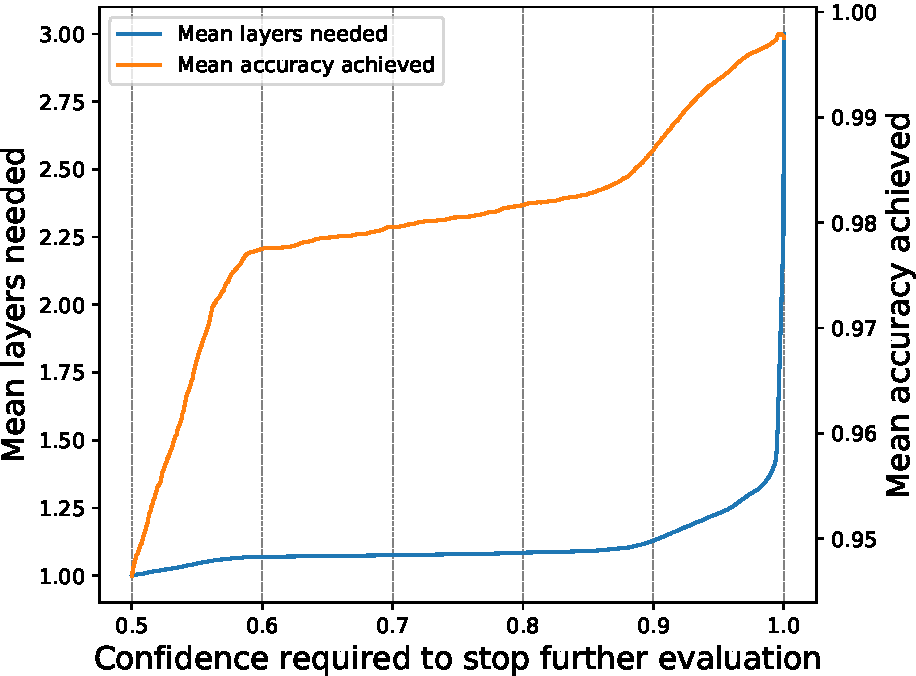
\includegraphics[width = 2.5in]{figures/conf-acc-17-3x128.pdf}} &
\subfloat[CIC-IDS17 (12 layers $\times$ 64 neurons).]{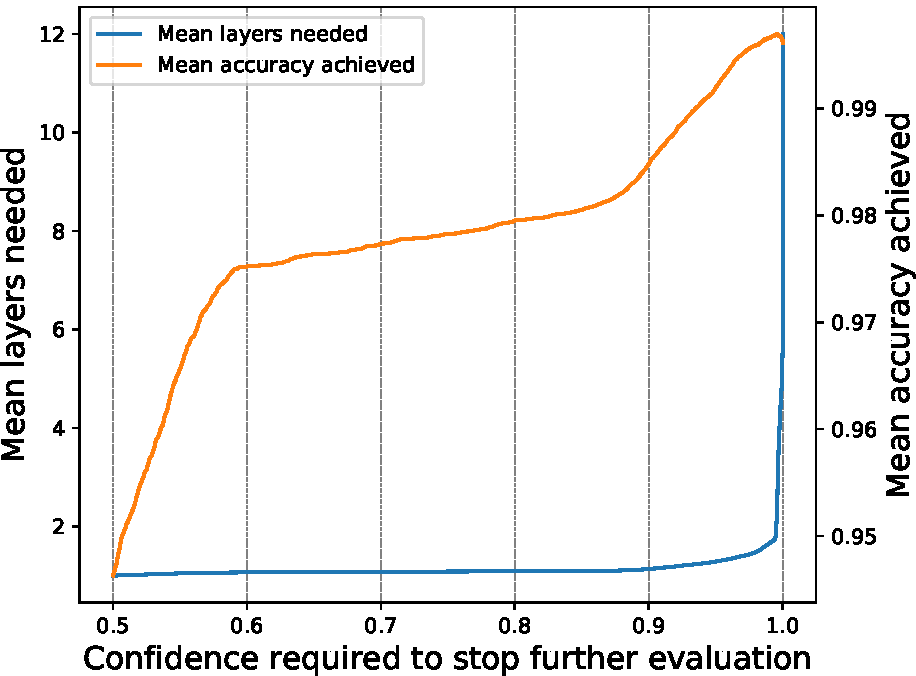
\includegraphics[width = 2.5in]{figures/conf-acc-17-12x64.pdf}}\\
\subfloat[UNSW-NB15 (3 layers $\times$ 128 neurons).]{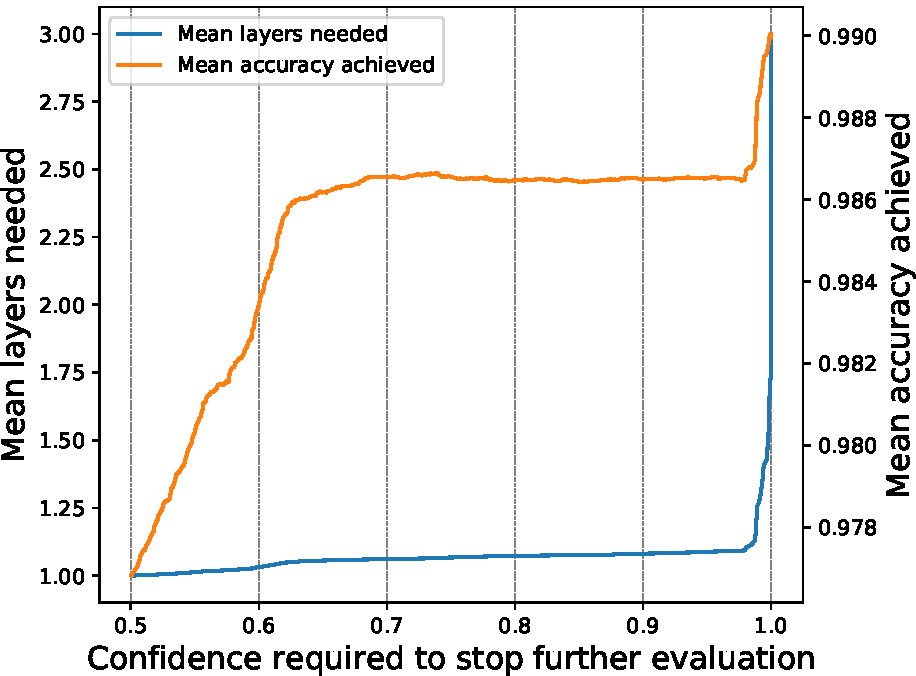
\includegraphics[width = 2.5in]{figures/conf-acc-15-3x128.pdf}} &
\subfloat[UNSW-NB15 (12 layers $\times$ 64 neurons).]{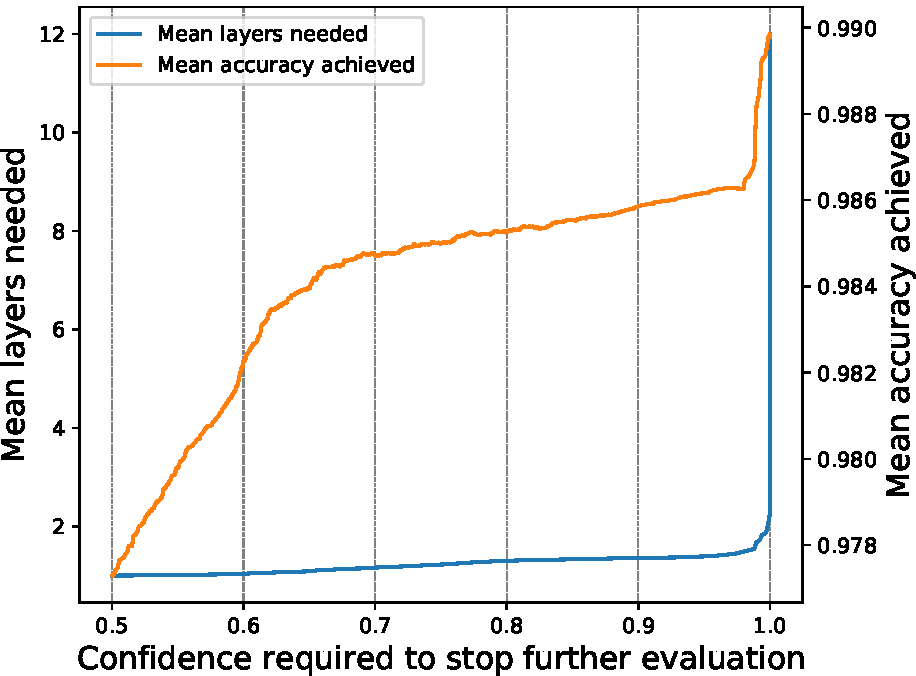
\includegraphics[width = 2.5in]{figures/conf-acc-15-12x64.pdf}}
\end{tabular}
\caption{Confidence threshold effect on accuracy and number of needed layers.}
\label{fig:confidence}
\end{figure*}

\begin{figure}
\center
\begin{tabular}{cccc}
\subfloat[CIC-IDS17 (12 layers $\times$ 64 neurons).]{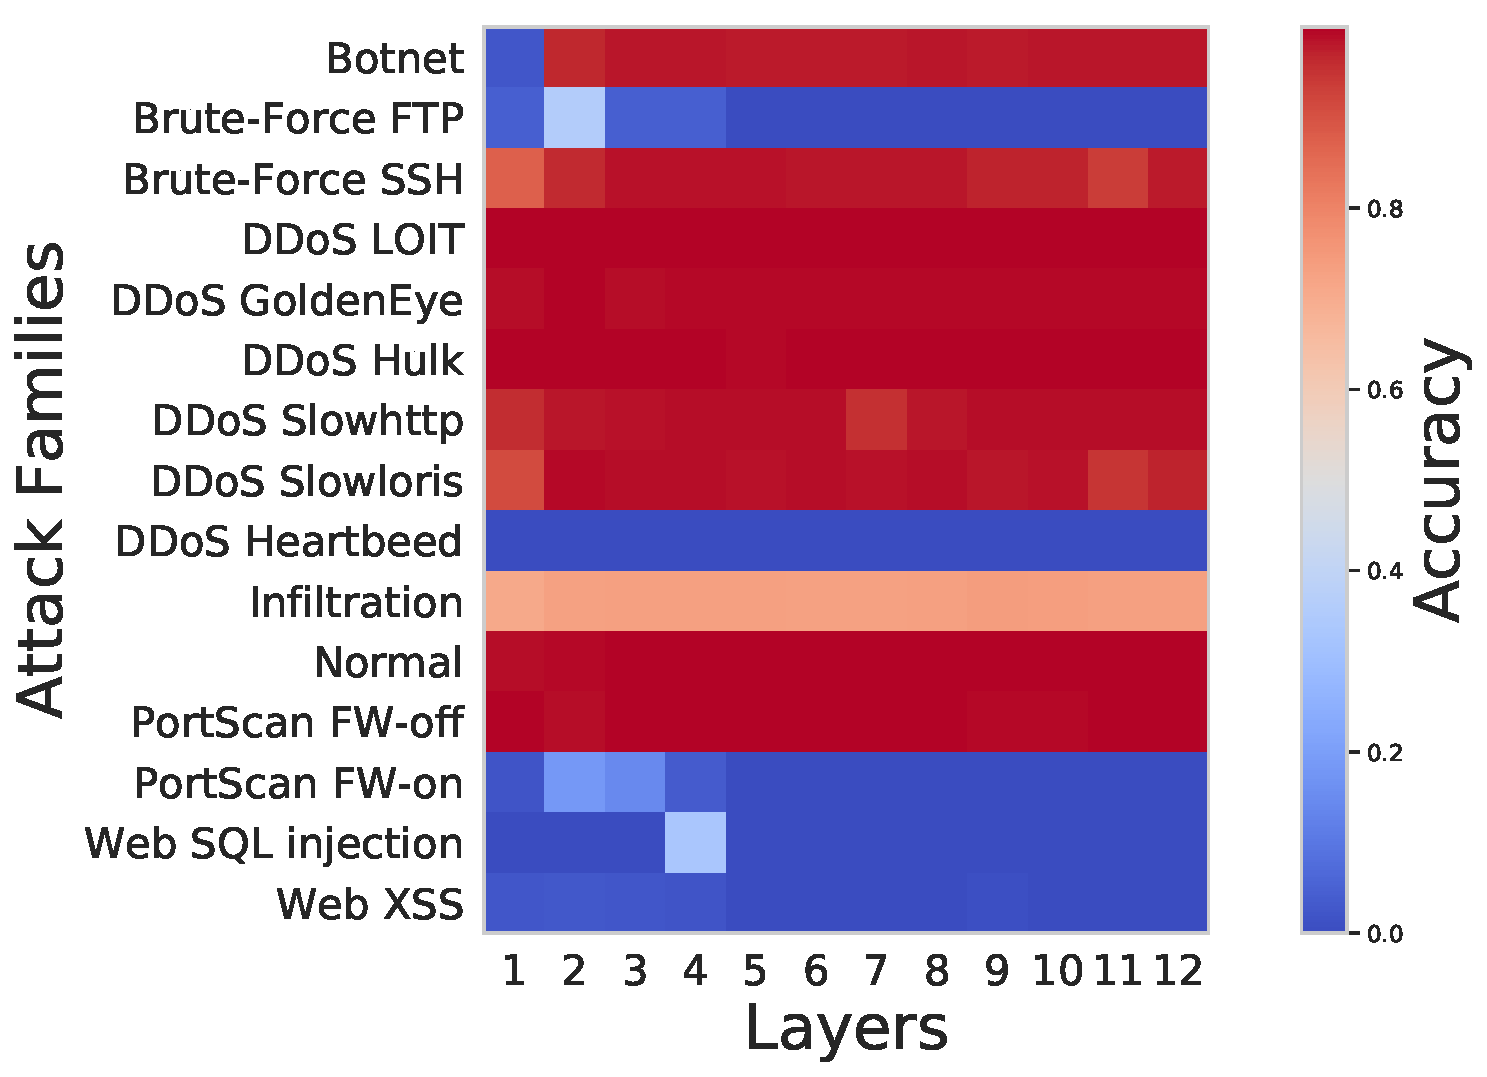
\includegraphics[width = 4in]{figures/multiclass17.pdf}} &
\subfloat[UNSW-NB15 (12 layers $\times$ 64 neurons).]{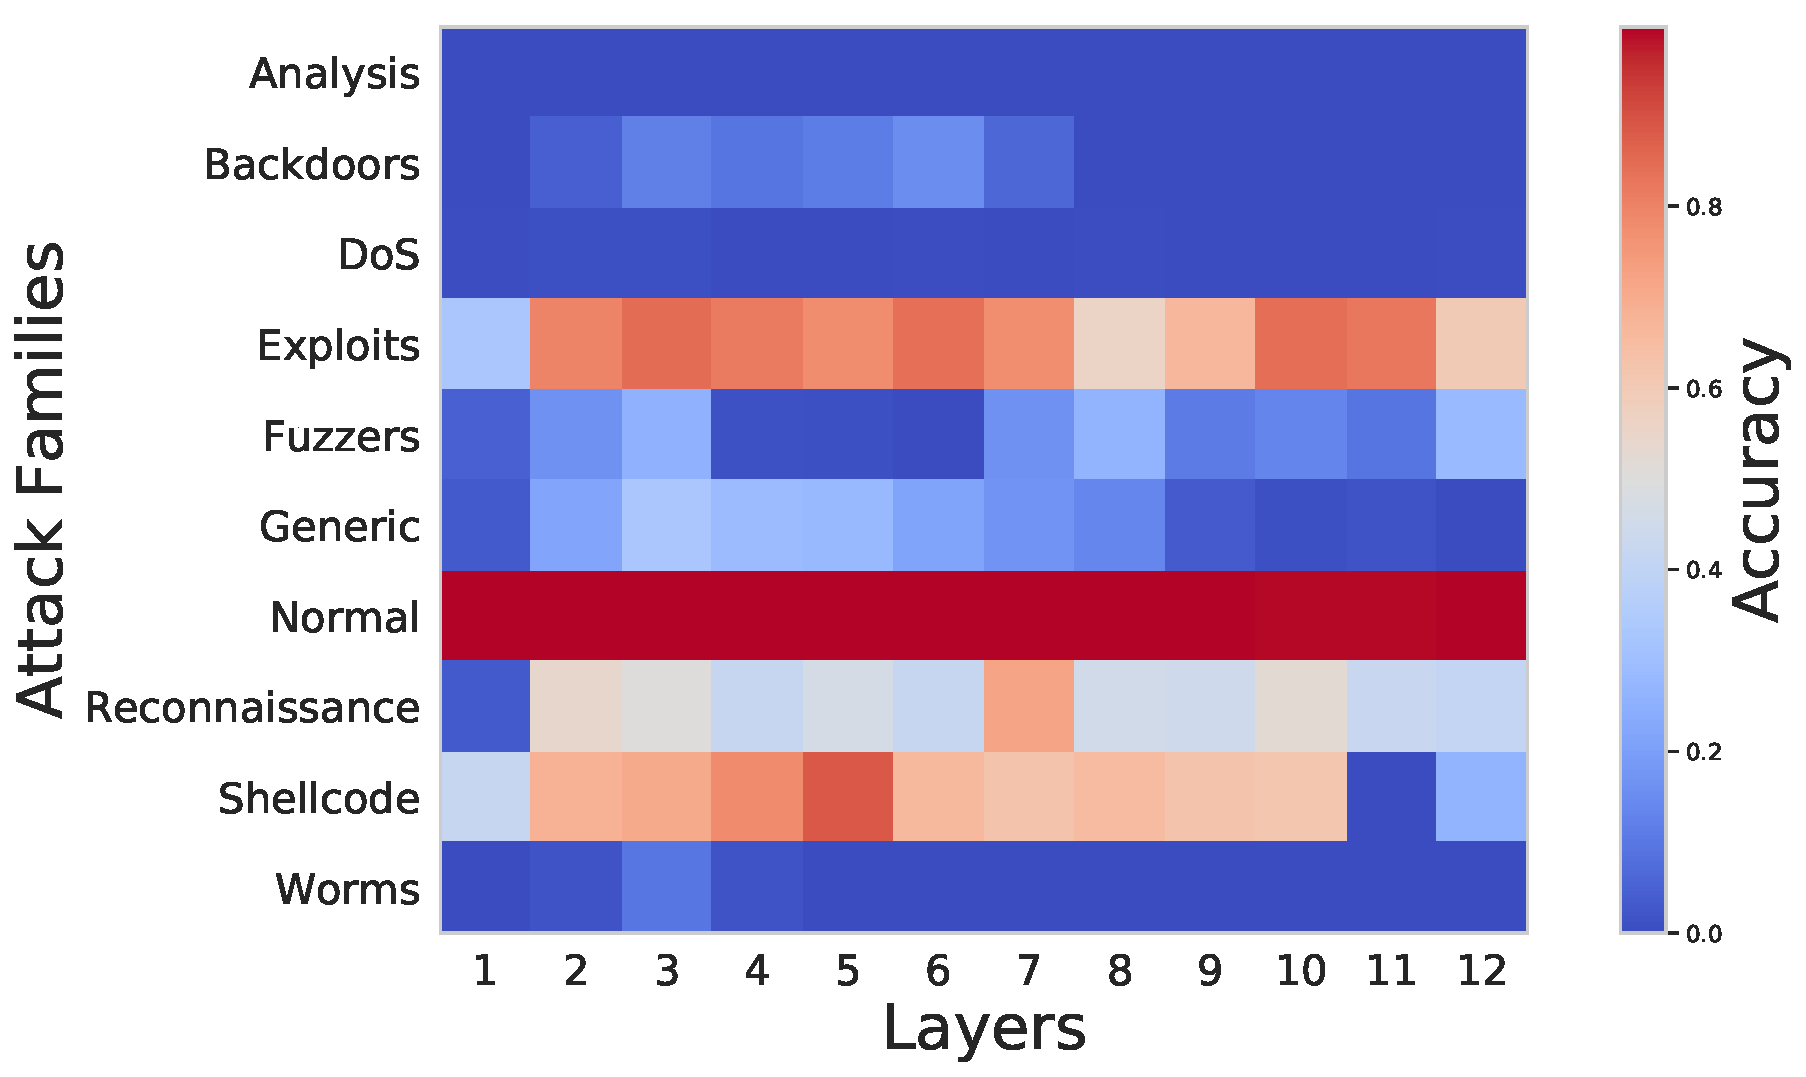
\includegraphics[width = 3in]{figures/multiclass15.pdf}}
\end{tabular}
\caption{Accuracy plot multiclass.}
\end{figure}

\textbf{Optimal Confidence Threshold.}
During deployment, the optimum confidence threshold is set by the user and plays a role in the overall achieved accuracy. Setting the threshold too low can cause the network to make decisions at an early stage, thereby gaining resources but achieving low accuracy. Similarly, setting the threshold too high can cause the network to skip the proper layers and thus always use the last one. The desired confidence level can therefore be obtained during the training phase by determining on the basis of the desired accuracy as shown in Figure \ref{fig:confidence}.

\subsubsection{Comparability to FNNs}
\label{comparability_to_fnns}


\begin{table}

\centering
\begin{tabular}{ccrc}
\toprule
\textbf{Dataset} & \textbf{Variant*} & \textbf{\gls{ffnn}} & \textbf{EagerNet (last)} \\
\midrule
\multirow{2}{*}{CIC-IDS17} & Binary & 0.989 & 0.993 \\
 & Multiclass & 0.920 & 0.979 \\
\midrule
\multirow{2}{*}{UNSW-NB15} & Binary & & \\
 & Multiclass & & \\
\midrule

\end{tabular}
\vspace{1ex}

{\raggedright * All architectures consist of 10 layers $\times$ 64 neurons in addition to input and output layers. \par}
\caption{Accuracy scores.}


\end{table}

\subsubsection{What Did the Network Learn?}
% why from 512 to 32







\section{Conclusion}


\section*{Acknowledgements}
The Titan Xp used for this research was donated by the NVIDIA Corporation.

\bibliographystyle{IEEEtran}
\bibliography{biblio}

\end{document}
